\documentclass{article}

% if you need to pass options to natbib, use, e.g.:
%\PassOptionsToPackage{numbers, compress}{natbib}
% before loading nips_2017
%
% to avoid loading the natbib package, add option nonatbib:
\usepackage[nonatbib,final]{nips_2017}

%\usepackage{nips_2017}

% to compile a camera-ready version, add the [final] option, e.g.:
%\usepackage[final]{nips_2017}

\usepackage[utf8]{inputenc} % allow utf-8 input
\usepackage[T1]{fontenc}    % use 8-bit T1 fonts
\usepackage{hyperref}       % hyperlinks
\usepackage{url}            % simple URL typesetting
\usepackage{booktabs}       % professional-quality tables
\usepackage{amsfonts}       % blackboard math symbols
\usepackage{nicefrac}       % compact symbols for 1/2, etc.
\usepackage{microtype}      % microtypography
\usepackage{algorithm}
\usepackage[noend]{algpseudocode}
\usepackage{shortcuts}
\usepackage{bm}
\usepackage[usenames,dvipsnames]{color}
\usepackage{amsmath,amsthm,amssymb,parskip,setspace,tabularx, wrapfig,float,enumerate} 
\usepackage{tikz, setspace, subfig, grffile}
\usepackage{subfig}



\usetikzlibrary{bayesnet}

\title{Mapping Gaussian Process Priors
\\ to Bayesian Neural Networks}

% The \author macro works with any number of authors. There are two
% commands used to separate the names and addresses of multiple
% authors: \And and \AND.
%
% Using \And between authors leaves it to LaTeX to determine where to
% break the lines. Using \AND forces a line break at that point. So,
% if LaTeX puts 3 of 4 authors names on the first line, and the last
% on the second line, try using \AND instead of \And before the third
% author name.

\author{
  Daniel Flam-Shepherd \\
  University of Toronto \\
  \texttt{ danielfs@utstat.utoronto.ca} \\
  \And
  James Requeima  \\
  University of Cambridge \\
  \texttt{jrr4l@cam.ac.ukl} \\
  \And
  David Duvenaud \\
  University of Toronto \\
  \texttt{duvenaud@cs.toronto.edu} \\
}

\begin{document}

\maketitle


\section{Introduction and Motivation}
What defines a reasonable prior to use when forming and training Bayesian models? 
 Recent work, such as \cite{hsp} seek to improve priors over network parameters, by applying
 a horseshoe prior over preactivations of a Bayesian neural network (BNN) to 
effectively turn off weights that do not explain the data. Our goal with this work
is to consider priors in function space as well. 

It is difficult to incorporate meaningful prior information about functions to be 
modeled by BNNs since priors are generally specified over the network parameters. 
Often, normal distributions are placed over the weights for convenience and 
are interpreted as a bias toward less complex functions via smaller weights. 
Gaussian processes, on the other hand, have a elegant mechanism for incorporating 
prior beliefs about the underlying function - specifying the mean and covariance functions.
However, Gaussian Processes have scalability limitations making Bayesian neural networks 
a more practical model in large data settings. 
In our work, we present an approach to specify a more principled prior for 
Bayesian Neural Networks that can leverage the well studied kernel design techniques from Gaussian process regression.


We consider matching the prior of a Bayesian neural network $\pbnn (\bm f |\bm \phi )$
to the prior of a Gaussian process $\pgp (\bm f  ) $ 
 by minimizing their approximate KL divergence via 
some data distribution of interest $\X \sim p(\X)$. 
We minimize this divergence with respect to the initial variational parameters $\bm \phi$ 
of the proposal distribution $q(\B w |\bm \phi)$. 
These variational parameters 
$\bm \phi^* = \{ \bm \mu _{\bm \phi}^* , \log \bm \sigma _{\bm \phi} ^* \} $ 
yield a prior on the BNN weights 
$p(\B w|\bm \phi^* ) = \N (\B w |\bm \mu _{\bm \phi}^* , \bm \sigma _{\bm \phi} ^* )$. 
Then, variational inference allows us to perform approximate inference in our BNN using this more 
principled prior. We describe the implementation of both steps and demonstrate its success in the following sections. 

\begin{figure}[h]\centering
\subfloat[BNN ]{\centering
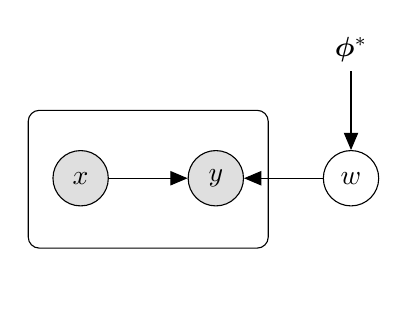
\begin{tikzpicture}[-latex, auto, l/.style={draw,thick,dashed}]
  \node[obs]                               (x) {$\B  x $};
  \node[below=of x]                               (s) {};
  \node[obs, right=of x]                   (y) {$\B  y $};
  \node[latent,right= of y]            (w) {$\B w$};
  \node[above= of w]                    (t) {$\bm \phi ^*$};
  

  % Connect the nodes
  \edge{x}{y};
  \edge{t}{w};
  \edge{w}{y};
  %\path[l] (x) edge [ bend left =40]node[left] {} (f);
        
  % Plates
  \plate[inner sep=.3cm, minimum size=1.75cm, ,yshift=.1cm] {} {(x)(y)} {} ;
\end{tikzpicture}
}
\hspace*{2.5cm}
\subfloat[GP ]{\centering
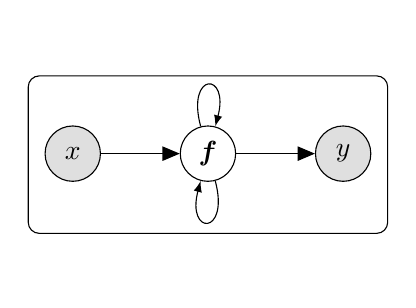
\begin{tikzpicture}[-latex, auto, l/.style={draw,thick,dashed}]
  \node[obs]                               (x) {$\B  x $};
  \node[below=of x]                               (s) {};
  \node[latent, right=of x]                (f) {$\bm f$};
  \node[obs, right=of f]                   (y) {$\B  y $};
  \node[above=of f] (d) {};
  \node[below=of f] (b) {};


  % Connect the nodes
  \path (f) edge [loop above, looseness=10] (f);
  \path (f) edge [loop below, looseness=10] (f);
  \edge{x}{f};
  \edge{f}{y};
   \plate[inner sep=.2cm, minimum size=2cm,yshift=.1cm] {} {(x)(y)} {} ;
 \end{tikzpicture}
}
\caption{ (a) and (b) display the graphical models of a BNN and GP.
} \label{fig:1}
\end{figure}


\newpage

\section{Mapping a GP prior to BNN prior}

In this section we describe the procedure used to minimize the KL divergence of  
the BNN prior distribution over functions $\pbnn (\bm f |  \bm \phi ) $ and
the GP prior distribution over functions  
$\pgp (\bm f ) \equiv \mathcal {G} \mathcal {P} (\bm f  | \bm 0, \B K )$ 
where $\B K$ is the Grahm matrix of the kernel or covariance function chosen. 
\begin{align}
    \mathcal K (\bm \phi)&= 
    \kl [\pbnn (\bm f |  \bm \phi ) \mid   \pgp (\bm f )] \\
    &= \int\pbnn (\bm f |  \bm \phi ) \log \BB{\frac{\pbnn (\bm f |  \bm \phi ) }{   \pgp (\bm f )}} d\bm f  \\
    &= -\entropy [\pbnn (\bm f |  \bm \phi ) ] 
       - \E_{\pbnn (\bm f |  \bm \phi ) } [\log \pgp (\bm f  ) ]    
\end{align}

We define our first stochastic optimization objective $\elbo _\X (\bm \phi)$ 
by approximating the KL divergence between these infinite dimensional distributions 
by taking expectations over some data distribution $p(\X)$, explicitly : 
$ \elbo _\X (\bm \phi) \equiv \E _{\X \sim p(\X)} [ \mathcal K (\bm \phi) ] $ . 
This allows us to prioritize where in the input space we want
 $\pbnn (\bm f |  \bm \phi ) \sim \pgp (\bm f  ) $. We have :
\begin{align}
\elbo _\X (\bm \phi)  = -\E _{\X \sim p(\X)} \entropy [\pbnn (\bm f (\X) |  \bm \phi ) ] 
	  			           - \E _{\X \sim p(\X)} \E_{\pbnn (\bm f (\X) |  \bm \phi ) } [\log \pgp (\bm f (\X) ) ]    
\end{align}

Both terms in equation (4) are intractable and force us to use some approximation. 
Since we are able to compute $\pgp (\bm f (\X))$ analytically, we can compute a Monte Carlo 
Estimate of the second term in (4):
\begin{align*}
	\E _{\X \sim p(\X)} \E_{\pbnn (\bm f |  \bm \phi ) } [\log \pgp (\bm f  ) ]  \approx  
  \frac{1}{S} \sum_{s=1}^S \E [\log \pgp (\bm f ^{(s)}(\X) ) ]
\end{align*}
where $\bm f ^{(s)}(\X) \sim \pbnn (\bm f | \X )$. 
For the entropy term in (4) we propose two estimation methods. 
\subsection{Estimate of entropy term using moment matching}

The first estimate we make involves the approximation that the prior distribution 
over functions for the BNN is a multivariate Gaussian distribution that takes form 
$\pbnn (\bm f (\X) |  \bm \phi ) \sim \N (\bm f | \bm \mu_{\bm f(\X) },\ \bm \Sigma _{\bm f(\X) } )$.  
In this case, the entropy term can be evaluated analytically over $p(\X) $ as 
$\entropy [\pbnn (\bm f (\X) |  \bm \phi ) ] = \half \log |2\pi e \bm \Sigma _{\bm f(\X) }| $ 
where we use the sample mean and covariance for 
$\bm \mu _{\bm f(\X) },\ \bm \Sigma _{\bm f(\X) }$ over $p(\X) $. 
This is a reasonable approximation because the overall goal in this work is push 
$\pbnn (\bm f |  \bm \phi ) \approx \pgp (\bm f  ) $ over $p(\X)$ 
and as $\pbnn (\bm f |  \bm \phi ) \to \pgp (\bm f  ) $ 
it will get more accurate. With this, the objective is  
\begin{align}
     \elbo _\X (\bm \phi) \approx
  -\half \log |\bm \Sigma _{\bm f(\X) }| -
  \frac{1}{S} \sum_{s=1}^S \E _{\X \sim p(\X)} [\log \pgp (\bm f ^{(s)}(\X) ) ]
\end{align}
We optimize this until convergence $ \bm \phi ^* =  \amin{\bm \phi}  \elbo _\X (\bm \phi ) $.
The details are in Algorithm 1. 

\begin{algorithm}
\caption{Optimization of the prior of the Bayesian neural net}
\begin{algorithmic}[1]
\State \textbf{Initialize} $\bm \phi =\{ \bm \mu _{\bm \phi} , \log \bm \sigma _{\bm \phi}  \}$
\While{ $\bm \phi$ not converged}
    \State $ \bm \epsilon ^{(s)} \sim p(\bm \epsilon) = \N (\B 0, \I) $
    \Comment{sample prior noise}
    \State $\B w ^{(s)} \gets t (\bm \phi, \bm \epsilon) = 
    \bm \mu _{\bm \phi} + \bm \sigma _{\bm \phi}\odot  \bm \epsilon ^{(s)}$
    \Comment{sample $S$ weights $\B w \sim q(\B w | \phi) $}
    \State $\X \gets ( \B x_1, \dots , \B x_n) \sim p(\B x_1, \dots , \B x_n )$ 
    \Comment{sample data} 
    \State $\bm f ^{(s)}(\X) \gets   f (\B X , \B w^{(s)} )$ 
    \Comment{sample $S$ functions $\bm f \sim \pbnn (\bm f |  \bm \phi )$}
    \State   $\B g _{\bm \phi} \gets \nabla _{\bm \phi} \elbo _{\tiny \X} (\bm \phi ) $
    \Comment{compute gradients of the objective}
    \State $\bm \phi \gets \text{adam}(\bm\phi , \B g _{\bm \phi} )$
    \Comment{update the parameters}
\EndWhile
\State \textbf{Return} $\bm \phi^*$
\end{algorithmic}
\end{algorithm}

The next section describes a formulation that allows to 
make an alternate approximation of the entropy term by considering the equivalent problem 
in observation space.
% ----------------------------------------------------------------------------------------------------- %

\newpage
\subsection{Estimate of entropy term by projecting into observation space}

Consider the equivalent problem in observation space by adding noise 
$\bm \epsilon \sim \N(\B 0, \sigma ^2 \I)$ to our functions 
$\B y =\bm f + \bm \epsilon$ so that we are minimizing the KL divergence of  
 $p (\B y |  \bm \phi ) $ : the BNN prior distribution over noisy observations 
 to the GP prior distribution over noisy observations   $\pgp (\B y )$.  
\begin{align}
    \mathcal K (\bm \phi)&= \kl [p (\B y |  \bm \phi ) \mid   \pgp (\B y )] 
    = -\entropy [p (\B y |  \bm \phi ) ] 
        - \E_{p (\B y |  \bm \phi ) } [\log \pgp (\B y ) ] 
\end{align}
Now we use Monte Carlo estimates of both $\entropy [p (\B y |  \bm \phi ) ]$ and
$ \E_{p (\B y |  \bm \phi ) } [\log \pgp (\B y | \bm \theta ) ]$  :
\begin{align}
        \mathcal K (\bm \phi) \approx \frac{1}{S} \sum_{s=1}^S \log p (\B y ^{(s)}|  \bm \phi) 
    									 -\frac{1}{S} \sum_{s=1}^S \log \pgp (\B y ^{(s)}) 	
\end{align}
where we are sampling $S$ times : $ \B y ^{(s)} \sim  p (\B y |  \bm \phi )$.
To estimate $  \log p (\B y ^{(s)}|  \bm \phi) $ we do approximate inference on an intermediate proposal 
distribution $r (\B w |\bm \lambda) $, where 
$\bm \lambda = \{ \bm \mu _{\bm \lambda} , \log \bm \sigma _{\bm \lambda}  \}$ 
are its variational parameters to be optimized. We then estimate  $  \log p (\B y ^{(s)}|  \bm \phi) $ 
using its ELBO $ \elbo _{\D _s } (\bm \lambda) $, optimized on data $\D _s =\{\X , \B y ^{(s)} \}$.
This is similar to Hierarchical variational models by \cite{hvm}. 
\begin{align}
 \log p (\B y ^{(s)}|  \bm \phi)  \geq \elbo _{\D _s } (\bm \lambda) 
 \equiv \E _{r(\B w |\bm \lambda )} \BB { \log p(\D_s | \B w)+\log p(\B w) - \log r(\B w |\bm \lambda )  } 
 \end{align}
where $\log p(\D_s | \B w) = \sum_i \log \N (\B y_i ^{(s)} | f(\B x_i, \B w), \sigma ^2\I )$ defines a parametric model. 
Once again we take expectations $p(\X)$ to define the objective 
$\elbo _\X (\bm \phi, \bm \lambda) \equiv \E _{\X \sim p(\X)} [\mathcal K  (\bm \phi) ]$  
by approximating the KL divergence between these infinite dimensional distributions. We obtain : 
\begin{align}
\elbo _\X (\bm \phi, \bm \lambda) 
 = \min _{\bm \phi} \frac{1}{S} \sum_{s=1}^S \max_{\bm \lambda}  \elbo _{\D _s} (\bm \lambda) 
 - \frac{1}{S} \sum_{s=1}^S  \E_{\X \sim p(\B X)} [\log \pgp (\B y ^{(s)}(\X))] 
\end{align}

We optimize (9) till convergence, this is described in the Algorithm 2. 

\begin{algorithm}
\caption{Mapping a GP prior to a BNN prior in observation space}
\begin{algorithmic}[1]
\State \textbf{Initialize} $\bm \phi =\{ \bm \mu _{\bm \phi} , \log \bm \sigma _{\bm \phi}  \}$
\While{ $\bm \phi$ not converged}
    \State $ \bm \epsilon ^{(s)} \sim p(\bm \epsilon) = \N (\B 0, \I) $
    \Comment{sample prior noise}
    \State $\B w ^{(s)} \gets \bm t( \bm \phi, \bm \epsilon^{(s)}) = \bm \mu _{\bm \phi} + \bm \sigma _{\bm \phi}\bm \epsilon ^{(s)}$
    \Comment{sample $S$ weights $\B w \sim q(\B w | \phi) $}
    \State $\X \gets (\B x_1, \dots , \B x_n) \sim p(\B x_1, \dots , \B x_n) \}$ 
    \Comment{sample from some data distribution} 
    \State $\bm f ^{(s)} \gets   f(\B X , \B w^{(s)} )$ 
    \Comment{sample $S$ functions from the BNN}
    \State $ \B y ^{(s)} \gets \bm f ^ {(s)}(\B X) +\bm \epsilon $ 
    \Comment{sample observations }
    \For{\texttt{each}  $\D _s =\{\X , \B y ^{(s)} \}$  \texttt{hold} $\bm \phi$ \texttt{constant and}}
         \State $\bm \lambda ^*_s \gets \argmax{\bm \lambda} \elbo _{\D _s } (\bm \lambda)  $
         \Comment{do approximate inference }
         \State $\log p(\B y^{(s}) \gets  \elbo _{\D _s } (\bm \lambda ^*_s)  $
         \Comment{estimate the marginal log likelihood}
    \EndFor
    \State  
    $\B g _{\bm \phi} \gets \nabla _{\bm \phi} \elbo _{\tiny \X} (\bm \phi, \bm \lambda )$
    \Comment{compute gradients of the kl}
    \State $\bm \phi \gets \text{adam}(\bm\phi ,\B g _{\bm \phi} )$
    \Comment{update the parameters}
\EndWhile
\State \textbf{Return} $\bm \phi^*$
\end{algorithmic}
\end{algorithm}
\subsection{Early Stopping}

Another rough approximation of (4) is to ignore the entropy term 
$\entropy [\pbnn (\bm f |  \bm \phi ) ]$ 
altogether, as it merely acts as a regularization term, so we avoid collapsing to a single high density value.
To address this issue, we found that early stopping works well in practice and yielded our best results. The results presented in the following section use early stopping and no entropy term. 

\newpage 

\section{Experiments with different kernels and activation functions}

We experiment with mapping GP priors (GPPs) with various covariance functions $k(x,x')$ to 
BNN priors that have various activation functions $a(x)$. We sample on order $10^3$
data from a uniform data distribution $\X \sim p(\X)$ about a symmetric interval (-10, 10). 
We use automatic differentiation software : \texttt{autograd} \cite{autograd, bbsvi} to 
compute gradients of our objective, which is optimized using adam \cite{adam}. 
In all experiments we work directly in function space 
and found that reasonable results can be found even when ignoring the entropy term 
$\entropy [p(\bm f)]$ altogether. Experiments are conducted on simple 1 or 2 layer neural 
networks. The prior proposal distribution on the BNN weights
is a diagonal Gaussian in all cases. In the following subsections, plots have color scheme:
$$ 
\textcolor{Green}{\bm f(\X) \sim \pgp (\bm f(\bm X))}, \ \
\textcolor{Red}{\bm f(\X) \sim \pbnn (\bm f(\bm X) | \bm \phi^*)}, \ \
\textcolor{Blue}{\bm f(\X) \sim \pbnn (\bm f(\bm X)) }  $$

\subsection{Linear and Softplus Experiments}

\begin{figure}[h]\centering
{
\includegraphics[width=.45\textwidth]{figs/linlin}
}
{
\includegraphics[width=.45\textwidth]{figs/rbfsoftplus}
}
\subfloat[]
{$\begin{aligned}
      k(x,x') &= xx'\\
         a(x) &= x
 \end{aligned}$}
\hspace{3.5cm}
\subfloat[]
{$\begin{aligned}
      k(x,x') &= e^{- (x-x')^2/50 }\\
         a(x) &= \log (1+e^x)
 \end{aligned}$}
\caption{In (a) we map a GPP with a linear kernel to a linear model (Bayesian Linear regression), 
the optimized prior samples extend from the origin just as the GPP samples do.
In (b) we map a GP prior with a RBF kernel to a BNN prior with a softplus activation function, 
the optimized samples have been mapped near the range of the GPP samples and almost as curvy 
as the GPP samples.
} \label{fig:1}
\end{figure}


\subsection{Experiments with rbf hyperbolic tan activations}

\begin{figure}[h]\centering
{
\includegraphics[width=.45\textwidth]{figs/rbfrbf}
}
{
\includegraphics[width=.45\textwidth]{figs/rbftanh}
}
\subfloat[]
{$\begin{aligned}
      k(x,x') &= e^{- (x-x')^2/2}\\
         a(x) &= e^{-x^2}
 \end{aligned}$}
\hspace{3cm}
\subfloat[]
{$\begin{aligned}
      k(x,x') &= e^{- (x-x')^2/50 }\\
         a(x) &= \tanh x
 \end{aligned}$}
\caption{ In (a) and (b) we map GP priors with a RBF kernel to BNNs with a RBF and tanh activation functions
It is clear that the optimized samples have taken on the curveness of the GPP samples} \label{fig:1}
\end{figure}

\newpage 

\subsection{Experiments with periodic kernels and activations}

\begin{figure}[h]\centering
{
\includegraphics[width=.45\textwidth]{figs/persin}
}
{
\includegraphics[width=.45\textwidth]{figs/persin2}
}
\subfloat[]
{$\begin{aligned}
      k(x,x') &= e^{-2\sin^2 (\pi| x-x'|) }\\
         a(x) &= \sin x
 \end{aligned}$}
\hspace{2.5cm}
\subfloat[]
{$\begin{aligned}
      k(x,x') &= e^{-2\sin^2 (\pi| x-x'|) /25 }\\
         a(x) &= \sin x
 \end{aligned}$}
\caption{  In (a) and (b) we map GPPs with periodic kernels to BNNs with sin activation functions.
The periodic structure of the GPP samples has been mapped to the optimized BNN samples.} \label{fig:1}
\end{figure}

\subsection{Experiments with other kernels}

\begin{figure}[h]\centering
{
\includegraphics[width=.45\textwidth]{figs/rqrbf}
}
{
\includegraphics[width=.45\textwidth]{figs/perrfbsin1}
}
\subfloat[]
{\hspace{1.0cm} 
$\begin{aligned}
      k(x,x') &= (1+(x-x')^2/6)^{-3}\\
         a(x) &=  e^{-x^2}
 \end{aligned}$}
\subfloat[]
{\hspace{1.0cm} 
$\begin{aligned}
      k(x,x') &= e^{-2\sin^2 (\pi| x-x'|) /25 }e^{- (x-x')^2/2 }\\
         a(x) &= \sin x
 \end{aligned}$}
\caption{In (a) we map a GPP with a rational cubic kernel to a BNN prior, the optimized samples have taken on 
the ''wigglyness'' of the prior samples especially away from the origin (the middle).
 In (b) we map a GPP with a locally periodic kernel to a BNN prior, the optimized samples take on both 
 the ''local wigglyness'' and the periodicity of the functions from the GPP} \label{fig:1}
\end{figure}


\section{Inference using the optimized prior}

Next we use the optimized parameters $\bm \phi^*$ 
found by minimizing the kl of the  $\pbnn (\bm f |\bm \phi )$
to $\pgp (\bm f  ) $  in a prior on the weights  
$p(\B w|\bm \phi ^*) =\N ( \B w |  \bm \mu _{\bm \phi} ^*,  \bm \sigma _{\bm \phi}^*) $. 
when maximizing the ELBO $ \elbo _\D (\bm \varphi ) \leq \log p(\D) $. 
\begin{align}
    \elbo _\D (\bm \varphi ) 
    =  \entropy [ q (\B w | \bm \varphi)] + 
        \E _{q (\B w | \bm \varphi)} \BB{ \log p (\D | \B w )  + \log p (\B w | \bm \bphi^* ) } 
\end{align}
Where $ \D =\{\B y, \X \} $ is the training data, $\bm \varphi =\{ \bm \mu_{\tiny\bm \varphi} , \log \bm \sigma _{\tiny \varphi} \} $ are the variational parameters of the approximation  
$q(\B w | \bm \varphi) = \N (\B w |\bm \mu_{\tiny\bm \varphi} , \bm \sigma _{\tiny \varphi} )$ 
to the true posterior on the weights $p(\B w |\D )$. Which we can sample from using reparameterization trick \cite{vae,sbpdgm}
 $\B w ^{(\ell)} = \bm t (\bm \varphi, \bm \epsilon)= \bm \mu _{\bm \varphi} + \bm \sigma _{\bm \varphi}\bm \epsilon ^{(\ell)} $.
Thus we can obtain unbiased stochastic gradients of the ELBO
with respect to the variational parameters. 
\newpage 

\subsection{Experiments on toy data}
We test our model (blue) on 2 different toy problems. We work directly in function space and 
use algorithm one, and we found that no entropy term estimate was necessary for reasonable results.
We compare to a BNN (blue) using a standard
normal prior distribution on the weights and 
to the posterior of a Gaussian process (green).  The BNNs are trained using Bayes by Backprop \cite{wunn}.
For both Gaussian process priors,  the kernel is the RBF covariance function. 
The observations $y$ are sampled by passing some data sampled uniformly 
through a function $f(x)$ and adding some Gaussian noise $\epsilon \sim \N (0, \sigma^2) $.
We use $\sigma =1$. The networks are all 2 layer with rbf activations as well. 
In the following plots the previous color scheme also applies 
$$ 
\textcolor{Green}{\bm f(\X) \sim \pgp (\bm f | \D )}, \ \
\textcolor{Red}{\bm f(\X) \sim \pbnn (\bm f(\bm X) |\varphi^*, \bm \phi^*)}, \ \
\textcolor{Blue}{\bm f(\X) \sim \pbnn (\bm f(\bm X)|\varphi^*) }  $$
\vspace{-0.5cm}  
\begin{figure}[h]   
    \hspace{2cm} $f(x) =x\sin x/10$ \hspace{4cm}  $f(x)= e^{-x^2/2} $

    \centering
    \includegraphics[width=.48\textwidth]{figs/xsinxgp}
    \includegraphics[width=.48\textwidth]{figs/expxgp}
    \includegraphics[width=.48\textwidth]{figs/xsinxgppbnn} 
    \includegraphics[width=.48\textwidth]{figs/expxgppbnn}    
    \includegraphics[width=.48\textwidth]{figs/xsinxbnn}    
    \includegraphics[width=.48\textwidth]{figs/expxbnn}       
    \caption{Plots of the 3 posteriors for 2 different functions.
    Different shades of color correspond to deciles of the predictive density 
    $ p(f(x_i)) $. The samples from this density are a slightly different shade 
    of green, red, and blue. The darkest is the mean. 
Notice that the mean and uncertainty bands of the posterior trained with the optimized prior
closer resembles the uncertainty of the Gaussian process. 
This demonstrates that our method of approximating a GP prior via a BNN can successfully 
transfer characteristics of the GP posterior to the BNN posterior as well. }
    \label{fig:my_label}
\end{figure}





\newpage

\section{Limitations}

In the previous sections we demonstrate the success of our proposed objective in completing the set out
task of mapping the properties of a Gaussian process prior to a Bayesian neural network prior.
However, there remain significant limitations of our method. We describe them below.

We found that we could not map GP priors to BNNs with certain activation functions, for example 
we could only map a GP prior with a linear kernel to a BNN with Relu activation functions at any capacity.
In this case, the BNN could not, at any capacity, learn the smoothness or periodic properties of any 
more interesting GP prior. 

As well, we could not map the properties of a GP prior with a periodic kernel to a BNN that did not 
have a periodic activation function. Our experiments focused on mapping properties of GP priors to BNNs 
with configurations that could reasonably learn those properties, for example periodic kernels to BNN priors 
with periodic activation functions.

We did not find an accurate estimator of the entropy term in our objective, as a result, training BNN priors
to behave like GP priors was difficult and was negatively hampered by lack of a accurate regularization term. 
Furthermore, rough estimates of the entropy term did not stabilize or improve these difficulties. Also, working 
in observation space with a more accurate estimation of the entropy term introduced another set of difficulties 
brought on by the mini max objective. As a consequence, we found that ignoring the entropy term and performing 
early stopping worked best. 

\begin{wrapfigure}{r}{0.6\textwidth}
  \begin{center}
    \includegraphics[width=0.58\textwidth]{figs/overfit}
  \end{center}
  \caption{An example of extreme overtraining}
\end{wrapfigure}

Often, without the entropy term, samples from the optimized BNN prior would take on the properties of the GP prior then gradually flatten and lose the desired properties. On the other hand, with the entropy term the samples would sometimes blow up. There was no stable regime where we could obtain consistent convergence. This would sometimes result in optimized samples which over emphasize the characteristics of the GP prior. 
An interesting example of this is displayed in Figure 7 where the red optimized samples take on an extremely local periodic behaviour later in training, while the samples of the GP prior being mapped do not have such a extreme periodic behavior.  



\section{Conclusions and Future Work}

In this work, we formulate a method for mapping a Gaussian process prior to a Bayesian neural network prior. 
This is done in effort to transfer interesting properties of functions sampled from a GP prior to functions
sampled from a Bayesian neural network prior. In this regard, we can implicitly think about priors in BNNs 
in function space rather than parameter space and overcome the limits that this entails. We demonstrate our method 
on a variety of kernels and activation functions, and gage its impact on posterior inference in simple toy examples.
All together, while there are important described limitations we establish that our method works throughout these
demonstrations and examples.                                                                                                                                                                                                                                                                                                          

This work attempts to build a small bridge between the flexible models of Bayesian non parametrics and the 
more scalable models of Bayesian deep learning. In future we seek to continue to build upon this idea of specifying 
priors in function space. The goal is to building more expressive Bayesian models where the prior 
better captures necessary prior beliefs and is more useful for posterior inference.  


\newpage

\subsubsection*{Acknowledgements}

The authors would like to thank Brian Ning and Guodong Zhang for helpful comments.


\bibliographystyle{unsrt}
\bibliography{refs}




\end{document}